\subparagraph*{Submission : }
\textit{Consider the general case in which the shop needs to optimize the prices and the assignment of promos to the customers in the case all the parameters need to be learnt.}\\

The problem requires to find the optimal prices for the two items and to optimize the assignment of the promos, in the scenario where all the parameters need to be learnt.

\subsection*{Strategy}
We simulate the random arrival of the customers. We have used a TS learner, with a number of arms given by the product between the number of pricing candidates for the first item and the number of pricing candidates of the second item. We pull the learner to retrieve a superarm, that specifies the couple of prices of the two items. It is defined, for each superarm, a UCB matching learner, defining the number of samples required to learn the parameters and the value for which the reward is divided to. We evaluate, for each customer, the purchase of the first item at the suggested price. In case the customer buys the first item, we pull the matching from the UCB learner defined for the pulled superarm, and we do the same procedure of purchase for the second item at the proposal discounted price. Before the arrival of a new customer, we update the TS learner with the entire reward given by the two items, and the UCB learner with the reward of the second item. We have used the same two matrixes, in the same way of the previous request.

\subparagraph{Implementation} 
\begin{itemize}
	\item No seasonality, conversion rate do no change
	\item Number of customers per class is not known 
	\item Candidates for the \textit{Racing Skis} are: \{2110.0, 1900.0, 2420.0, 2690.00\}
	\item Candidates for the \textit{Racing Ski Helmet} are: \{360.0, 410.0, 530.0, 600.0\}
	\item Conversion rate associated with the first item is not known
	\item Conversion rate associated with the second item is not known
	\item Promotion assignment is not known 
\end{itemize}


\subparagraph{Optimal strategy}
In order to calculate the regret, we have defined the optimal solution in the following manner: for every possible combination of the candidates of the two item, we calculate the reward of the first item as the sum over the category of the product of the number of customers per category, the conversion rate of each category for the considered candidate price and the candidate price. We calculate a matrix for every possible matching, where every cell is equal to the product of the conversion rate of the first item releated to the considered customer category, the conversion rate of the second item releated to the discounted price given by the releated discounted price and the customer category, the number of customer for the considered category and the discounted price.
We retrieve the optimal matching by using the linear sum assignment function on the matrix previous calculated. The sum of the reward of the optimal matching provides the total reward of the second item. The highest reward related to the two pricing candidates and to the optimal matching is our optimal solution.
According to our candidates the optimal solution is:
\begin{itemize}
	\item Optimal price Racing Skis: 1900.0
	\item Optimal price Racing Ski Helmet: 410.0
	\item Optimal matching: Sport addicted: P0; Gifter: P2; Amateur: P3; Worried: P1
\end{itemize}
Days: 365\\
Experiments number: 3 \\

\subsection*{Results}
\begin{center}
	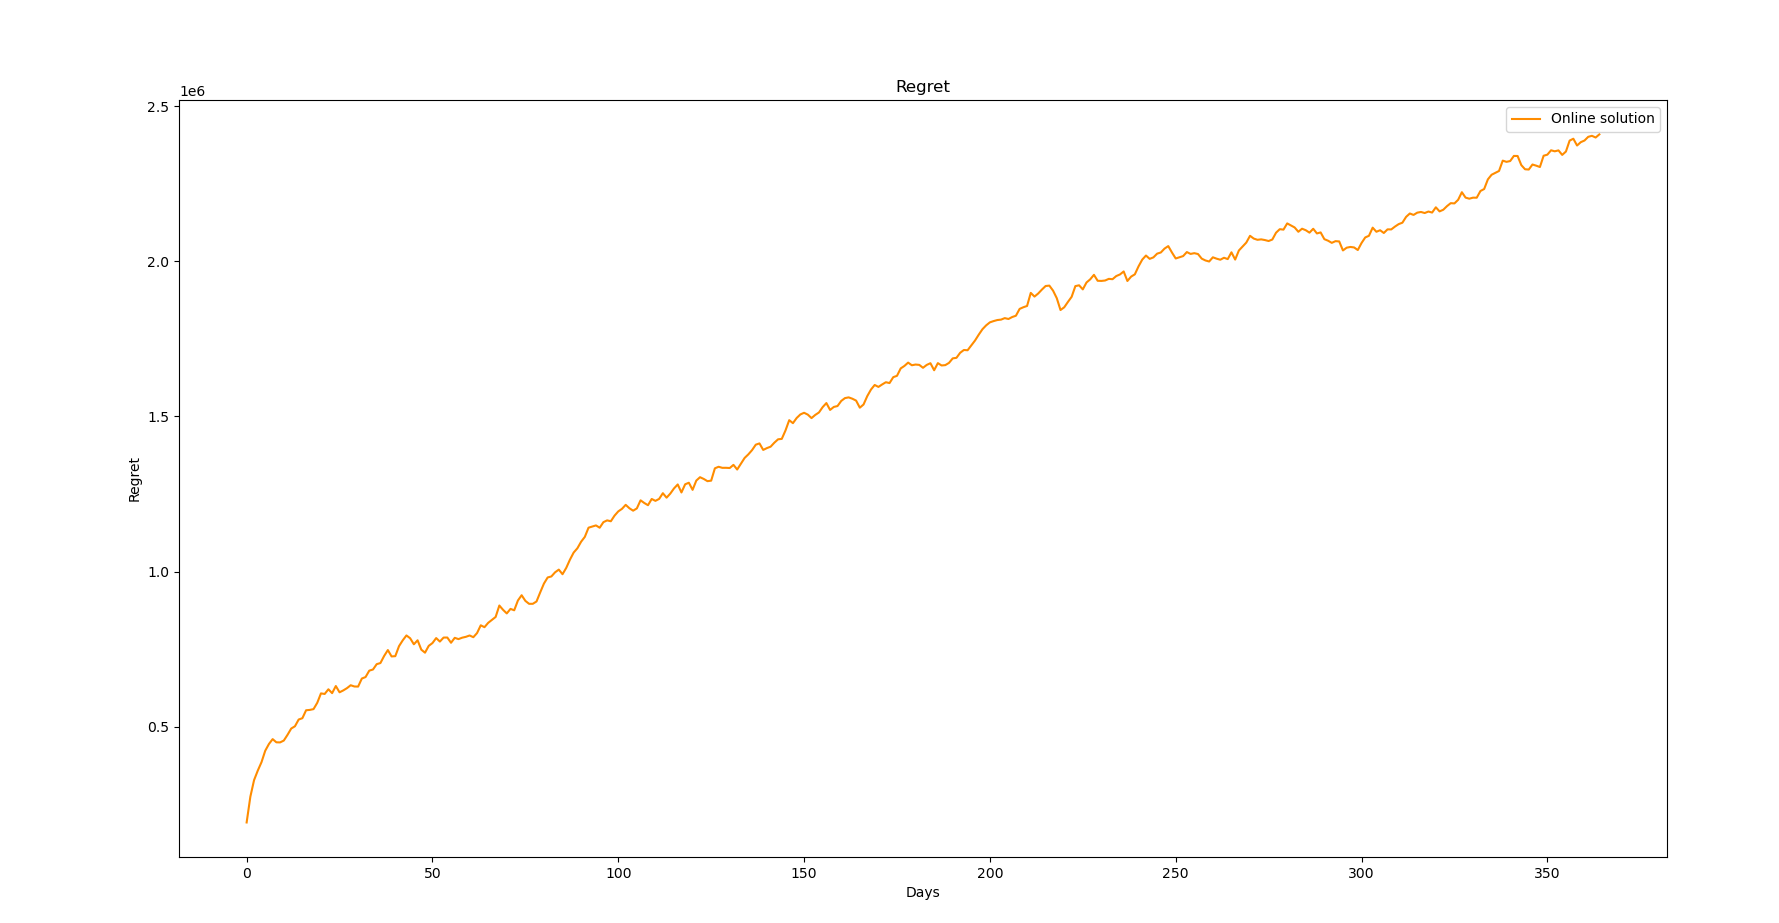
\includegraphics[scale=0.35]{Images/n6}
\end{center}

\subsection*{Considerations}
We can notice that the learners take more time to learn the optimal solutions both for pricing and matching. The cumulative regret is increasing quite linearly until the day 200th, after that, they start to stabilize on the optimal solutions. The cumulative regret still be jagged, because both the learner can pull random arms with some probabilty, this has impact on the curve.